\begin{flushright} {\tiny {\color{gray} python\_codes/fieldstone\_117/text.tex}} \end{flushright}

\lstinputlisting[language=bash,basicstyle=\small]{python_codes/fieldstone_117/keywords}

\begin{center}

\fbox{\textbf{\huge \color{teal} P}}
Codes at \url{https://github.com/cedrict/fieldstone/tree/master/python_codes/fieldstone_01}
\end{center}

\par\noindent\rule{\textwidth}{0.4pt}

{\sl This fieldstone was developed in collaboration with Lukas van de Wiel}. \index{contributors}{L. van de Wiel}

\par\noindent\rule{\textwidth}{0.4pt}
%%%%%%%%%%%%%%%%%%%%%%%%%%%%%%%%%%%%%%%%%%%%%%%%%%%%%%%%%%%%%%%%%%%%%%%%%%%%%%%%%%%%%%%%%%%%%%


%-------------------------------
\subsection*{The mesh}

The mesh(es) used in this \stone are obtained by means of the quilt mesher program written by Lukas. 

in quilt.f: 
elementType = Q4

in examples.f, in subroutine meshThirteenPatches:
nElemsBase=10


%-------------------------------
\subsection*{The benchmarks}

I have implemented five finite element pairs: $Q_1\times P_0$, $Q_2\times Q_1$, $Q_2 \times P_{-1}$,
$Q_3\times Q_2$, $Q_4\times Q_3$.
Note that unfortunately the vtu format does not allow the representation of $Q_3$ or $Q_4$ fields. 

Two benchmarks are implemented in the code: Donea \& Huerta (see Section~\ref{mms:dh}) and SolVi (see Section~\ref{mms:solvi}).
The first one is a manufactured solution which has a vertical and horizontal symmetry. As such the tailored mesh 
is of no use here. The second is of course why the mesher was developed in the first place: the viscosity contrast between 
inclusion and matrix aligns exactly with the mesh:

\begin{center}
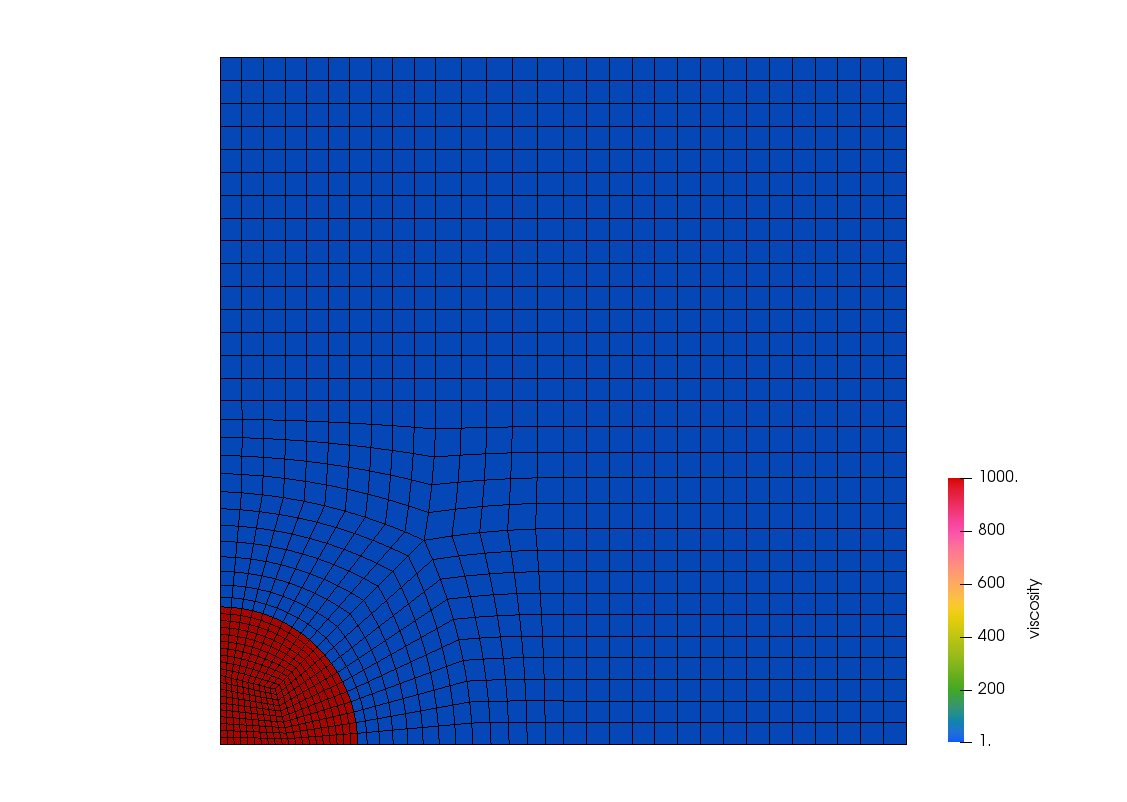
\includegraphics[width=5cm]{python_codes/fieldstone_117/images/visc}
\end{center}

 

dafuq is going on with Nxx Nyy ? 


do Q2P1 unmapped

do Q2(8)Q1


